\section{The Traditional Square of Opposition}

We have seen that conversion, obversion, and contraposition allow us to identify some valid one-premise arguments. There are actually more we can find out there, but investigating them is a bit more complicated. The original investigation made by the Aristotelian philosophers made an assumption that logicians no longer make.  To help you understand all sides of the issue, we will begin by looking at things in the traditional Aristotelian fashion, and then in the next section move on to the modern way of looking at things.

When Aristotle was first investigating these four kinds of categorical statements, he noticed they they conflicted with each other in different ways. If you are just thinking casually about it, you might say that ``No $S$ is $P$'' is somehow ``the opposite'' of ``All $S$ is $P$.'' But isn't the real ``opposite'' of ``All $S$ is $P$'' actually ``Some $S$ is not $P$''?

Aristotle, in his book \cite{Aristotle:interpretation}, notes that the real opposite of A is O, because one must always be true and the other false.  If we know that ``All dogs are mammals'' is true, then we know ``some dog is not a mammal'' is false. On the other hand, if ``All dogs are mammals'' is false then ``some dog is not a mammal'' must be true. Back on page \pageref{def:contradictory} we said that when two propositions must have opposite truth values they are called contradictories. Aristotle noted that A and O sentences are contradictory in this way. Forms E and I also form a contradictory pair. If ``Some dogs are mammals'' then ``No dogs are mammals'' is false, and if ``Some dogs are mammals'' is false, then ``No dogs are mammals'' is true.


\newglossaryentry{contraries}
{
name=contraries,
description={Two statements that can't both be true, but can both be false. A set two inconsistent sentences.}
}


Mood-A and mood-E statements are opposed to each other in a different way. Aristotle claimed that they can't both be true, but could both be false. Take the statements ``All dogs are strays'' and ``No dogs are strays.'' We know that they are both false, because some dogs are strays and others aren't. However, it is also clear that they could not both be true. When a pair of statements cannot both be true, but might both be false, the Aristotelian tradition says they are \textsc{\gls{contraries}}. \label{def:Contraries} Aristotle's idea of a pair of contraries is really just a specific case of a set of sentences that are \emph{inconsistent}, an idea that we looked at in Chapter \ref{chap:whatisformallogic}. (See page \ref{def:inconsistency})

\newglossaryentry{square of opposition}
{
name=square of opposition,
description={A way of representing the four basic propositions and the ways they relate to one another.}
}


These distinctions, plus a few other comments from Aristotle, were developed by his later followers into an idea that came to be known as the \textsc{\gls{square of opposition}} \label{def:Squareofopposition}. The square of opposition is simply the diagram you see in Figure \ref{fig:traditionalsquare}. It is a way of representing the four basic propositions and the ways they relate to one another.  As we said before, this way of picturing the proposition turned out to make a problematic assumption. To emphasize that this is no longer the way logicians view things, we will call this diagram the traditional square of opposition.

The traditional square of opposition begins by picturing a square with A, E, I, and O at the four corners. The lines between the corners then represent the ways that the kinds of propositions can be opposed to each other. The diagonal lines between A and O and between E and I represent contradiction. These are pairs of propositions where one has to be true and the other false. The line across the top represents contraries. These are propositions that Aristotle thought could not both be true, although they might both be false.

In Figure \ref{fig:traditionalsquare}, we have actually drawn each relationship as a pair of lines, representing the kinds of inferences you can make in that relationship. Contraries cannot both be true. So we know that if one is true, the other must be false. This is represented by the two lines going from a T to an F. Notice that there aren't any lines here that point from an F to something else. This is because you can't infer anything about contrary statements if you just know that one is false. For the contradictory statements, on the other hand, we have drawn double-headed arrows. This is because we know both that the truth of one statement implies that the other is false and that the falsity of one statement implies the truth of the other.

\newglossaryentry{subcontraries}
{
name=subcontraries,
description={Two categorical statements that cannot both be false, but might both be true.}
}

Contraries and contradictories just give us the diagonal lines and the top line of the square. There are still three other sides to investigate. Form I and form O are called \textsc{\gls{subcontraries}}. \label{defSubcontraries} In the traditional square of opposition, their situation is reversed from that of A and E. Statements of forms A and E cannot both be true, but they can both be false. Statements of forms I and O cannot both be false, but they can both be true. Consider the sentences ``Some people in the classroom are paying attention'' and ``Some people in the classroom are not paying attention.'' It is possible for them both to be true. Some people are paying attention and some aren't. But the two sentences couldn't both be false. That would mean that everyone in the room was neither paying attention nor not paying attention. But they have to be doing one or the other!

This means that there are two inferences we can make about subcontraries. We know that if I is false, O must be true, and vice versa. This is represented in Figure \ref{fig:traditionalsquare} by arrows going from Fs on one side to Ts on the other. This is reversed from the way things were on the top of the square with the contraries. Notice that this time there are no arrows going away from a T. This is because we can't infer anything about subcontraries if all we know is that one is true

\newglossaryentry{subalternation}
{
name=subalternation,
description={The relationship between a universal categorical statement and the particular statement with the same quality.}
}


The trickiest relationship is the one between universal statements and their corresponding particulars. We call this \textsc{\gls{subalternation}}. Both of the statements in these pairs could be true, or they could both be false. However, in the traditional square of opposition, if the universal statement is true, its corresponding particular statement must also be true. For instance, ``All dogs are mammals'' implies that some dogs are mammals. Also, if the particular statement is false, then the universal statement must also be false. Consider the statement ``Some dinosaurs had feathers.'' If that statement is false, if no dinosaurs had feathers, then ``All dinosaurs have feathers'' must also be false. Something like this seems to be true on the negative side of the diagram as well. If ``No dinosaurs have feathers'' is true, then you would think that ``some dinosaurs do not have feathers'' is true. Similarly, if ``some dinosaurs do not have feathers'' is false, then ``No dinosaurs have feathers'' cannot be true either.

In our diagram for the traditional square of opposition, we represent subalternation by a downward arrow for truth and an upward arrow for falsity. We can infer something here if we know the top is true, or if we know the bottom is false. In other situations, there is nothing we can infer.

Note, by the way, that the language of subalternation works a little differently than the other relationships. With contradiction, we say that each sentence is the ``contradictory'' of the other. The relationship is symmetrical. With subalternation, we say that the particular sentence is the ``subaltern'' of the universal one, but not the other way around.

People started using diagrams like this as early as the second century \textsc{ce} to explain Aristotle's ideas in \textit{On Interpretation} (See Parsons \cite*{Parsons1997}). Figure \ref{fig:apuleiussquare} shows one of the earliest surviving versions of the square of opposition, from a 9th century manuscript of a commentary on Aristotle attributed to the Roman writer Apuleius of Madaura. Although this particular manuscript dates from the 9th century, the commentary itself was written in the 2nd century, and copied by hand many times over before this one was made. Figure \ref{fig:majorsquare} shows a later illustration of the square, from a 16th century book by the Scottish philosopher and logician Johannes de Magistris.

\begin{figure}
\begin{center}
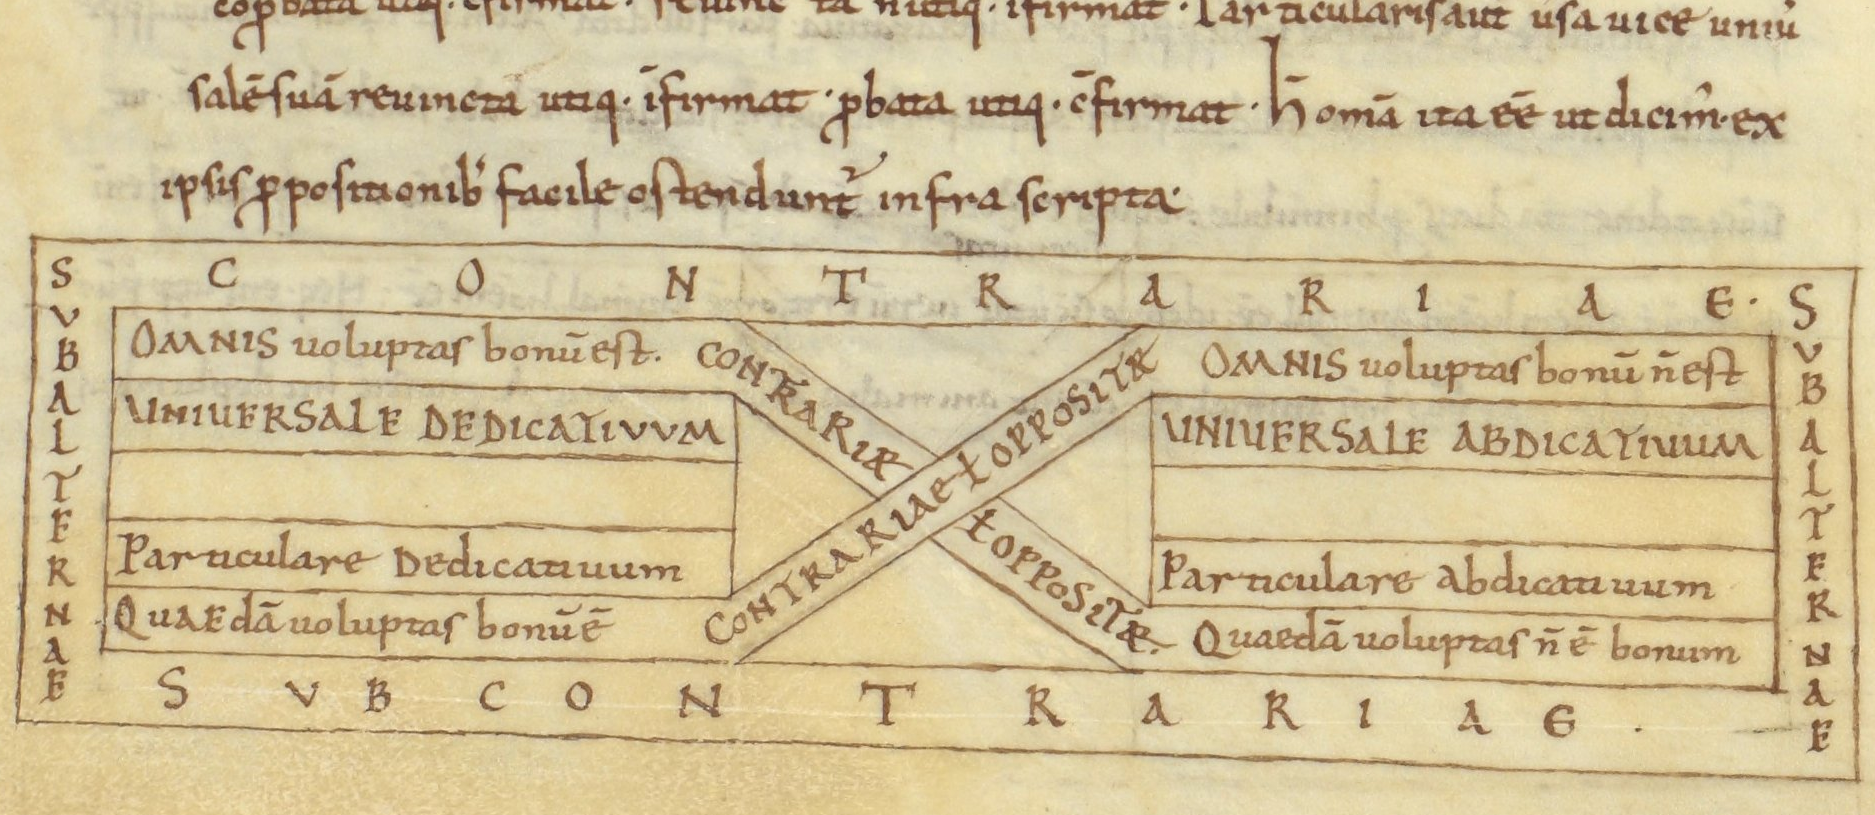
\includegraphics[scale=.4]{ljs101}
\end{center}
\caption{One of the earliest surviving versions of the square of opposition, from a 9th century manuscript that includes a commentary on Aristotle by the African writer Apuleius of Madaura (\cite{Apuleius1987}). The manuscript is held Lawrence J. Schoenberg collection (LJS 101) at the University of Pennsylvania, who have kindly put a facsimile online (\url{http://dla.library.upenn.edu/dla/medren/detail.html?id=MEDREN_5186550}.)  Screencap by J. Robert Loftis.}
\label{fig:apuleiussquare}
\end{figure}


\begin{figure}
\begin{center}
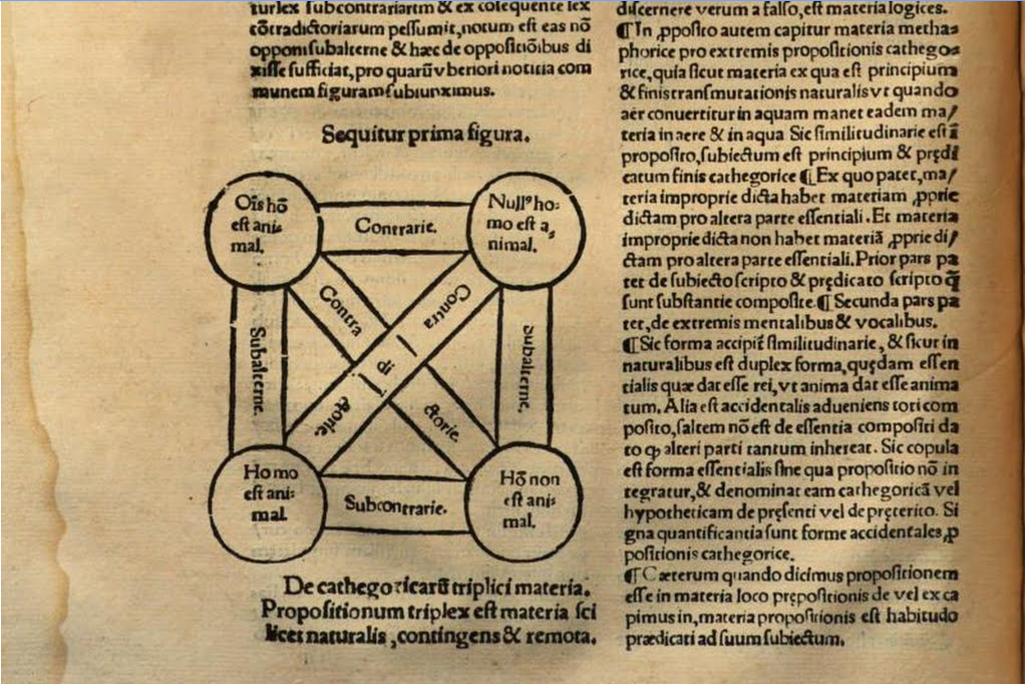
\includegraphics[scale=.5]{majorvenn2}
\end{center}
\caption{A 16th century illustration of the square of opposition from John Major's \textit{Introductorium Perutile in Aristotelicam Dialecticen} (\cite*[fol.L]{Major1527}). Screencap from Google Books by J.  Robert Loftis.}
\label{fig:majorsquare}
\end{figure}

As with the processes of conversion, obversion, and contraposition, we can use the traditional square of opposition to evaluate arguments written in canonical form. It will help us here to introduce the phrase ``It is false that'' to some of our statements, so that we can make inferences from the truth of one proposition to the falsity of another. This, for instance, is a valid argument, because A and O statements are contradictories.


\begin{kormanize}
\premise{ All humans are mortal.}
\conclusion{ It is false that some human is not mortal.}
\end{kormanize}

The argument above is an immediate inference, like the arguments we saw in the previous section, because it only has one premise. It is also similar to those arguments in that the conclusion is actually logically equivalent to the premise. This will not be the case for all immediate inferences based on the square of opposition, however. This is a valid argument, based on the subaltern relationship, but the premise and the conclusion are not logically equivalent.

\begin{kormanize}
\premise{ It is false that some humans are dinosaurs.}
\conclusion{  It is false that all humans are dinosaurs.}
\end{kormanize}


% ****************************************************
% * Existential Import and the Modern Square of Opposition    *
% ****************************************************

\section{Existential Import and the Modern Square of Opposition}
\label{sec:ExistentialImport}

The traditional square of opposition seems straightforward and fairly clever. Aristotle made an interesting distinction between contraries and contradictories, and subsequent logicians developed it into a nifty little diagram. So why did we have to keep saying things like ``Aristotle thought'' and ``according to the traditional square of opposition.'' What is wrong here?

The traditional square of opposition goes awry because it makes assumptions about the existence of the things being talked about. Remember that when we drew the Venn diagram for ``All $S$ are $P$,'' we shaded out the area of $S$ that did not overlap with $P$ to show that nothing could exist there. We pointed out, though, that we did not put a little x in the intersection between $S$ and $P$. Statements of the form A ruled out the existence of one kind of thing, but they did not assert the existence of another. The A proposition, ``All dogs are mammals,'' denies the existence of any dog that is not a mammal, but it does not assert the existence of some dog that is a mammal. But why not? Dogs obviously do exist.

The problem comes when you start to consider categorical statements about things that don't exist, for instance ``All unicorns have one horn.'' This seems like a true statement, but unicorns don't exist. Perhaps what we mean by ``All unicorns have one horn'' is that \emph{if} a unicorn existed, \emph{then} is would have one horn. But if we interpret the statement about unicorns that way, shouldn't we also interpret the statement about dogs that way? Really all we mean when we say ``All dogs are mammals'' is that if there were dogs, then they would be mammals. It takes an extra assertion to point out that dogs do, in fact, exist.

\newglossaryentry{existential import}
{
name=existential import,
description={An aspect of the meaning of a statement that which is present if the statement can only be true when the objects it describes exist.}
}

\newglossaryentry{vacuous truth}
{
name=vacuous truth,
description={The kind of truth possessed by statements that do not have existential import and refer to objects that do not exist.}
}

The issue we are discussing here is called existential import. A sentence is said to have \textsc{\gls{existential import}} \label{def:Existential_import} if it asserts the existence of the things it is talking about. Figure \ref{fig:existential_import} shows the two ways you could draw Venn diagrams for an A statement, with the x, as in the traditional interpretation, and without, as in our interpretation. If you interpret A statements in the traditional way, they are always false when you are talking about things that don't exist. So, ``All unicorns have one horn'' is false in the traditional interpretation. On the other hand, in the modern interpretation all statements about things that don't exist are true. ``All unicorns have one horn'' simply asserts that there are no multi-horned unicorns, and this is true because there are no unicorns at all. We call this \textsc{\gls{vacuous truth}}. Something is vacuously true \label{def:Vacuous_truth} if it is true simply because it is about things that don't exist. Note that \emph{all} statements about nonexistent things become vacuously true if you assume they have no existential import, even a statement like ``All unicorns have more than one horn.'' A statement like this simply rules out the existence of unicorns with one horn or fewer, and these don't exist because unicorns don't exist. This is a complicated issue that will come up again starting in Chapter \ref{chap:SL} when we consider conditional statements. For now just assume that this makes sense because you can make up any stories you want about unicorns.



Any statement can be read with or without existential import, even the particular ones. Consider the statements ``Some unicorns are rainbow colored'' and ``Some unicorns are not rainbow colored.'' You can argue that both of these statements are true, in the sense that if unicorns existed, they could come in many colors. If you say these statements are true, however, you are assuming that particular statements do not have existential import. As Terence Parsons (\cite*{Parsons1997}) points out, you can change the wording of particular categorical statements in English to make them seem like they do or do not have existential import. ``Some unicorns are not rainbow colored'' might have existential import, but ``not every unicorn is rainbow colored'' doesn't seem to.

So what does this have to do with the square of opposition? A lot of the claims made in the traditional square of opposition depend on assumptions about which statements have existential import. For instance, Aristotle's claim that contrary statements cannot both be true requires that A statements have existential import. Think about the sentences ``All dragons breathe fire'' and ``no dragons breathe fire.'' If the first sentence has no existential import, then both sentences could actually be true. They are both ruling out the existence of certain kinds of dragons and are correct because no dragons exist.

In fact, the entire traditional square of opposition falls apart if you assume that all four forms of a categorical statement have existential import. Parsons (\citep{Parsons1997}) shows how we can derive a contradiction in this situation. Consider the I statement ``Some dragons breathe fire.'' If you interpret it as having existential import, it is false, because dragons don't exist. But then its contradictory statement, the E statement ``No dragons breathe fire'' must be true. And if that statement is true, and has existential import, then its subaltern, ``Some dragon does not breathe fire'' is true. But if it has existential import, it can't be true, because dragons don't exist. In logic, the worst thing you can ever do is contradict yourself, but that is what we have just done. So we have to change the traditional square of opposition.

 The way some textbooks talk about the problem, you'd think that for two thousand years logicians were simply ignorant about the problem of existential import and thus woefully confused about the square of opposition, until finally George Boole wrote \textit{The Laws of Thought}\cite{Boole1854} and found the one true solution to the problem. In fact, there was an extensive discussion of existential import from the 12th to the 16th centuries, mostly under the heading of the ``supposition'' of a term. Very roughly, we can say that the supposition of a term is the way it refers to objects, or what we now call the ``denotation'' of the term.\cite{Read2002}
 So in ``All people are mortal'' the supposition of the subject term is all of the people out there in the world. Or, as the medievals sometimes put it, the subject term ``supposits'' all the people in the world.

At least some medieval thinkers had a theory of supposition that made the traditional square of opposition work. Terrance Parsons (\citep{Parsons1997}, \citep{Parsons2008}) has argued for the importance of one solution, found most clearly in the writings of William of Ockham. Under this theory, affirmative forms A and I had existential import, but the negative forms E and O did not. We would say that a statement has existential import if it would be false whenever the subject or predicate terms refer to things that don't exist. To put the matter more precisely, we would say that the statement would be false whenever the subject or predicate terms ``fail to refer.'' Linguistic philosophers these days prefer say that a term ``fails to refer'' rather than saying that it ``refers to something that doesn't exist,'' because referring to things that don't exist seems impossible.

In any case, Ockham describes the supposition of affirmative propositions the same way we would describe the reference of terms in those propositions. Again, if the proposition supposes the existence of something in the world, the medievals would say it ``supposits.''  Ockham says ``In affirmative propositions a term is always asserted to supposit for something. Thus, if it supposits for nothing the proposition is false'' (\citep{Ockham1343}, 206). On the other hand, failure to refer or to supposit actually supports the truth of negative propositions: ``in negative propositions the assertion is either that the term does not supposit for something or that it supposits for something of which the predicate is truly denied. Thus a negative proposition has two causes of truth'' (\citep{Ockham1343}, 206).

So, for Ockham, affirmative statements about nonexistent objects are false. ``All unicorns have one horn'' and ``Some unicorns are rainbow colored'' are false, because there are no unicorns. Negative statements, on the other hand, are vacuously true. ``No unicorns are rainbow colored'' and ``No unicorns have one horn'' are both true. There are no rainbow colored unicorns out there, and no one horned unicorns out there, because there are no unicorns out there. The O statement ``Some unicorns are not rainbow colored'' is also vacuously true. This might be harder to see, but it helps to think of the statement as saying ``It is not the case that every unicorn is rainbow colored.''

This way of thinking about existential import leaves the traditional square of opposition intact, even in cases where you are referring to nonexistent objects. Contraries still cannot both be true when you are talking about nonexistent objects, because the A proposition will be false, and the E vacuously true. ``All dragons breathe fire'' is false, because dragons don't exist, and ``No dragons breathe fire'' is vacuously true for the same reason. Similarly, subcontraries cannot both be false when talking about dragons and whatnot, because the I will always be false and the O will always be true. You can go through the rest of the relationships and show that similar arguments hold. \label{proving_trad_square}

Boole proposed a different solution, which is now taken as the standard way to do things. Instead of looking at the division between positive and negative statements, Boole looked at the division between singular and universal propositions. The universal statements A and E do not have existential import, but the particular statements I and O do have existential import. Thus all particular statements about nonexistent things are false and all universal statements about nonexistent things are vacuously true.

John Venn was building on the work of George Boole. His diagrams avoided the problems that Euler had by using a Boolean interpretation of mood-A statements, where they really just assert that something is impossible. In fact, the whole system of Venn diagrams embodies Boole's assumptions about existential import, as you can see in Figure \ref{fig:fourvenns}. The particular forms I and O have you draw an x, indicating that something exists. The other two forms just have us shade in regions to indicate that certain combinations of subject and predicate are impossible. Thus A and E statements like ``All dragons breathe fire'' or ``No dragons are friendly'' can be true, even though no dragons exist.

Venn diagrams doesn't even have the capacity to represent Ockham's understanding of existential import. We can represent A statements as having existential import by adding an x, as we did on the right hand side of Figure \ref{fig:existential_import}. However, we have no way to represent the O form without existential import. We have to draw the x, indicating existence. We don't have a way of representing O form statements about nonexistent objects as vacuously true.

The Boolean solution to the the question of existential import leaves us with a greatly restricted form of the square of opposition. Contrary statements are both vacuously true when you refer to nonexistent objects, because neither have existential import. Subcontrary statements are both false when you refer to nonexistent objects, because they do have existential import. Finally, the subalterns of vacuously true statements are false, while on the traditional square of opposition they had to be true. The only thing remaining from the traditional square of opposition is the relationship of contradiction, as you can see in Figure \ref{fig:modernsquare}.
